\documentclass[../notes.tex]{subfiles}

\pagestyle{main}
\renewcommand{\chaptermark}[1]{\markboth{\chaptername\ \thechapter\ (#1)}{}}
\stepcounter{chapter}

\begin{document}




\chapter{DNA}
\section{DNA Synthesis and Transcription}
\begin{itemize}
    \item \marginnote{10/4:}DNA binding proteins.
    \begin{itemize}
        \item Interact with major grooves of DNA to achieve sequence specificity.
        \item Example: Transcription factors that have to turn a gene on or off.
        \item Such proteins often do this with two primary motifs: The leucine zipper and the zinc finger.
        \begin{itemize}
            \item Leucine zipper: Less programmable.
            \item Zinc finger: More programmable. Contains 1+ zinc ion coordinated by cysteine and histidine. One zinc finger interacts with three base pairs.
        \end{itemize}
        \item With the scale of our genome, you typically need a sequence of 15-18 base pairs to achieve specificity. That's 5-6 zinc fingers.
        \item When they were discovered, zinc fingers were thought to be a possibility for genome editing.
    \end{itemize}
    \item DNA structure and binding modes.
    \begin{itemize}
        \item DNA binding proteins may also interact with the minor groove (to achieve some specificity), electrostatically with the phosphate backbone (usually not sequence-specific), and intercalation (a flat molecule splits two base pairs a bit and inserts itself in).
    \end{itemize}
    \item Minor groove: Deep and narrow.
    \begin{itemize}
        \item Minor groove binding can involve electrostatics, hydrophobic burial, and hydrogen bonding.
        \item Minor groove binding can be site specific. There are some features you can take advantage of, e.g., being flat and flexible.
    \end{itemize}
    \item Pyrrole-Imidazole-Hydroxypyrrole (Py/Im/Hp) Polyamides.
    \begin{itemize}
        \item Pioneered by the Dervan lab at CalTech.
        \item Minor-groove binding polyamides consisting of three aromatic ring amino acids.
        \item Flexible because of the amides.
        \item Eight-ring pyrrole-imidazole polyamides achieve affinities and specificities comparable to DNA-binding proteins.
        \item Cell-permeable molecules for gene-specific regulation \emph{in vivo}.
        \item Still not specific enough, though.
    \end{itemize}
    \item Minor groove-binding small molecules.
    \begin{itemize}
        \item Examples (not testable material): Hoechst 33258, DAPI, Distamycin, and Berenil.
        \begin{itemize}
            \item Distamycin in the minor groove. Distamycin is an antibiotic and it fits very well into the minor groove. Preference for A/T sequences.
            \item Hoechst 33258 in the minor groove. Also fits very well; uset to some extent to dye DNA, but more often in flow cytometry.
        \end{itemize}
        \item Common features (testable material):
        \begin{itemize}
            \item Flat (to slip into the minor groove).
            \item Small linked aromatic ring systems (to allow ring systems to make local adjustments).
            \item Curved (to match curvature of the minor groove).
            \item Positively charged (to interact with the phosphates).
            \item H-bond donors on concave face (to H-bond with acceptors on base pairs).
        \end{itemize}
    \end{itemize}
    \item Phosphate backbone binding.
    \begin{itemize}
        \item Driven by electrostatics.
        \begin{itemize}
            \item Ligands that bind this way are always cationic, binding depends strongly on salt concentration.
            \item Ions (\ce{Na+}, \ce{Mg^2+}, etc.)
        \end{itemize}
        \item Example: Biogenic polyamines (involved in a lot of biological processes).
        \begin{itemize}
            \item For example, putrescine is a positively charged polyamine. It is responsible for bad breath!
        \end{itemize}
        \item \textbf{Transfaction reagents} wrap around DNA and neutralize some of its negative charge to help it get into cells.
    \end{itemize}
    \item Intercalators.
    \begin{itemize}
        \item Example: Ethidium bromide (a toxic molecule used to stain DNA).
        \item Features in common:
        \begin{itemize}
            \item Extended aromatic systems (to provide extensive overlap with base pairs).
            \item Electron deficient (to complement regions of high electron density in base pairs).
        \end{itemize}
    \end{itemize}
    \item Intercalation requires structural rearrangement.
    \begin{itemize}
        \item The intercalator does disturb DNA structure a bit as it pushes base pairs farther apart, causing buckling in adjacent base pairs and a tilt in the helical axis.
        \item Because of this, intercalators can alter DNA replication.
    \end{itemize}
    \item Ethidium bromide as a DNA dye.
    \begin{itemize}
        \item Biochemical analysis of DNA (gel electrophoresis).
        \begin{itemize}
            \item Agarose is used for DNA strands over 300 bp. Bands greater than 100,000 bp are not resolved.
            \item Concentration of agarose can be increased to create a denser matrix, or decreased to create a less dense matrix.
            \item Larger molecules need a less dense matrix.
            \item Because DNA is negatively charged, it migrates to the cathode (+) of the electrophoresis system.
        \end{itemize}
        \item Ethidium bromide is toxic: It can act as a mutagen because it intercalates double-stranded DNA and, as mentioned, affects replication.
        \begin{itemize}
            \item If you add too much ethidium bromide into your PCR, it may not work (the polymerase may not be able to overcome it).
        \end{itemize}
        \item Safer options are offered by many biotech companies: sybr-green, sybr-gold, etc.
        \begin{itemize}
            \item Tang isn't sure how much safer these actually are.
            \item The common design is bigger molecules: Will still intercalate DNA, but will not penetrate the skin as easily.
        \end{itemize}
    \end{itemize}
    \item Summary.
    \begin{itemize}
        \item Several forms of DNA/RNA (most important ones: A-RNA and B-DNA).
        \item Unusual forms may also play an important role (e.g., G-quadruplex and tRNA).
        \item Molecules that interact with the DNA.
        \begin{itemize}
            \item Major grove interactions are sequence specific.
            \item Minor grove interactions can be sequence specific.
            \item Phosphate backbone/intercalation interactions are (typically) not sequence specific.
        \end{itemize}
    \end{itemize}
    \item This is the end of the previous lecture's slides.
    \item Now: Replication, transcription, translation, and nucleic acid catalysis.
    \item Overview.
    \begin{itemize}
        \item DNA replication in cells: DNA-templated synthesis of DNA.
        \item DNA repair in cells: Enzymatic repair of DNA mutations
        \item DNA transcription in cells: DNA-templated synthesis of RNA.
        \item Translation: Nucleic acid catalysis (difficult) and RNA-templated synthesis of proteins.
    \end{itemize}
    \item If you find the early topics above difficult, review the relevant sections of \textcite{bib:Lehninger}.
    \item DNA is synthesized/replicated by DNA polymerase.
    \begin{figure}[h!]
        \centering
        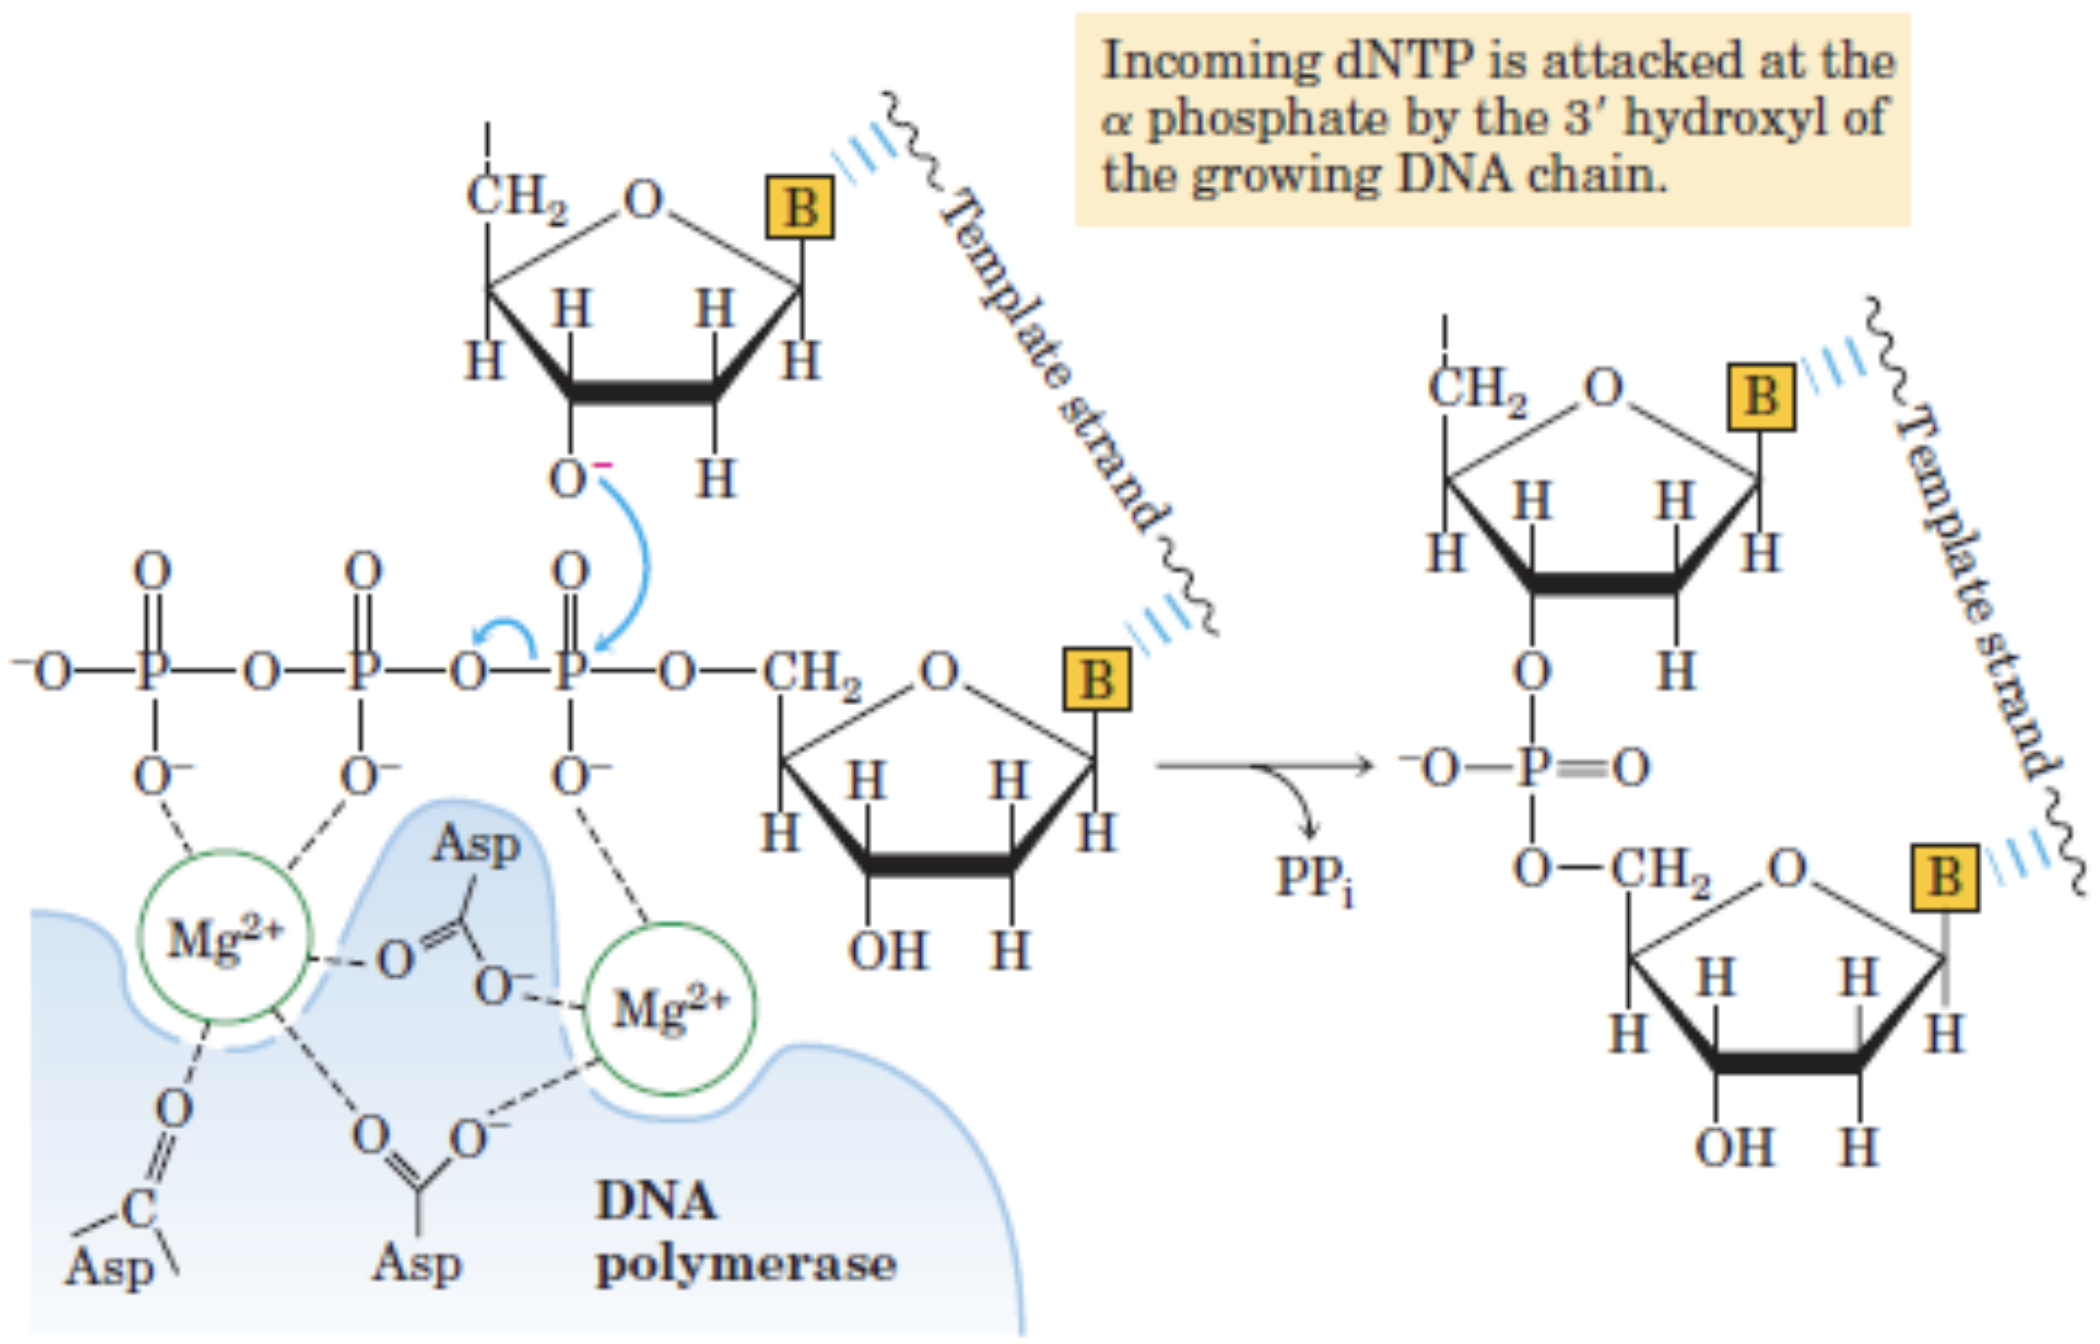
\includegraphics[width=0.6\linewidth]{../ExtFiles/DNASynMech.png}
        \caption{Mechanism of DNA synthesis.}
        \label{fig:DNASynMech}
    \end{figure}
    \begin{itemize}
        \item DNA polymerases require three components: A template, a primer, and dNTPs\footnote{Deoxynucleoside triphosphate} (N = A, T, G, or C).
        \item Mechanism: The 3' hydroxyl of the growing DNA chain attacks the $\alpha$ phosphate of the incoming dNTP via nucleophilic acyl substitution.
        \begin{itemize}
            \item Most textbooks will draw the electron pushing as a substitution reaction, but in reality, the double bond gets resolved, and then kicks back down to get rid of the $\beta$ and $\gamma$ phosphates.
            \item Energetically driven by the BDE of the dNTP, so as long as dNTP is abundant, the reaction can proceed.
        \end{itemize}
        \item In bacteria, this process can occur at a rate of 1000 bp/second.
        \begin{itemize}
            \item Our cells are slower.
        \end{itemize}
        \item Notice the presence here of magnesium (partially coordinated to aspartic acid) catalyzing the reaction as part of DNA polymerase.
        \begin{itemize}
            \item One \ce{Mg^2+} coordinates with the $\beta$ and $\gamma$ phosphates to stabilize them.
            \item The other coordinates with the $\alpha$ phosphate to stabilize the highly negatively charged nucleophilic acyl substitution intermediate.
        \end{itemize}
        \item DNA replication in \emph{E. coli} is highly accurate (error rate \numrange{e-9}{e-10}).
        \begin{itemize}
            \item Two reasons: Templated synthesis (error rate of \numrange{e-4}{e-5} \emph{in vitro}) and error correction mechanisms.
        \end{itemize}
        \item Templated synthesis is equivalent to having a 99.999\% yield in an organic reaction (which never happens).
        \item One error-correction mechanism bridging the gap from \num{e-5} to \num{e-10}: DNA polymerase "proofreads" even as it synthesizes DNA.
        \item Example procedure:
        \begin{itemize}
            \item Let C* be a rare tautomer of cytosine that pairs with A and is incorporated into the growing strand.
            \item Before the polymerase moves on, the C* reconverts to C and is now mispaired.
            \item The mispaired 3'-OH end of the growing strand blocks further elongation. DNA polymerase slides back to position the mispaired base in the $3'\to 5'$ exonuclease active site.
            \item The mispaired nucleotide is removed.
            \item DNA polymerase slides forward and resumes its polymerization activity.
        \end{itemize}
        \item Not every polymerase has this feature, but most high-fidelity ones do.
    \end{itemize}
    \item DNA replication in cells.
    \begin{itemize}
        \item DNA replication is semiconservative.
        \begin{itemize}
            \item Meselson-Stahl experiment, "the most beautiful experiment in biology."
        \end{itemize}
        \item DNA replication begins at an \textbf{origin} and proceeds \textbf{bidirectionally}.
        \item Bacterial chromosomes have a single point of origin; most other cells have multiple such points.
    \end{itemize}
    \item DNA replication requires many enzymes and protein cofactors.
    \begin{itemize}
        \item DNA replication in cells requires much more than solely polymerases.
        \item DNA replication in \emph{E. coli} requires 20 or more different enzymes and proteins, each performing a specific task.
        \item DNA replicase system (replisome): The entire complex is required for DNA replication.
        % \item Key proteins of the \emph{E. coli} replisome.
        % \begin{itemize}
        %     \item SSB: Single-stranded DNA binding protein. Stabilizes the exposed single stranded parts of DNA as it is unwound and before its complement is synthesized.
        %     \item Helicase: Unwinds DNA; continuously expands the origin.
        %     \item Primase: Synthesizes a primer. Regardless of whether it's DNA- or RNA-templated synthesis, it's always primed.
        %     \item DNA polymerase vs. ligase: DNA polymerase is the main one; Ligase bridges the lagging strands together.
        % \end{itemize}
    \end{itemize}
    \item Three identifiable phases of DNA replication in \emph{E. coli}.
    \begin{enumerate}
        \item Initiation.
        \begin{itemize}
            \item Five repeats of 9 bp (R sites) for DnaA binding; A = T rich DNA unwinding element (DUE).
            \item DnaA binding, DUE denaturing, DnaB helicase loading, then ready for the next phase.
            \item Initiation is the only phase of DNA replication that is known to be precisely regulated (replication occurs only once in each cell cycle). You don't want the daughter cells to have multiple unneeded copies of the genome.
        \end{itemize}
        \item Elongation.
        \begin{itemize}
            \item Single-stranded DNA-binding protein (SSB) stabilizes the regions denatured by helicase.
            \item Two distinct but related operations: Leading strand synthesis and lagging strand synthesis.
            \item Lagging strand synthesis requires RNA primers (synthesized by primase) to form Okazaki fragments.
            \begin{itemize}
                \item Regardless of whether it's DNA- or RNA-templated synthesis, it's always primed.
            \end{itemize}
            \item After completion of an Okazaki fragment, RNA primer is removed and replaced with DNA by DNA polymerase I, and the remaining nick is sealed by DNA ligase.
        \end{itemize}
        \item Termination.
        \begin{itemize}
            \item Ter sequences: Trap for the bidirectional replication of DNA by forming Tus-Ter complex --- prevent overreplication by one replication folk when the other folk is abnormally delayed or halted.
            \item \textbf{Catenane} formation: Bidirectional replication of DNA meets at the end.
            \item DNA topoisomerase IV: Separate the catenated chromosomes into normal chromosomes for the daughter cells.
        \end{itemize}
    \end{enumerate}
    \item \textbf{Catenane}: A mechanically interlocked molecular architecture consisting of two or more interlocked macrocycles\footnote{Recall the discussion of this in \emph{The Knot Book}!}.
    \item We don't have to remember every protein; Tang just wants to show us.
    \begin{itemize}
        \item Note that the ones that she did show us, though, are all involved in elongation; initiation and termination require additional proteins.
        \item Also, new proteins are still being discovered.
        \item DNA replication in eukaryotic cells is both similar and more complex than in \emph{E. coli}.
    \end{itemize}
    \item Mutations happen constantly in DNA.
    \begin{itemize}
        \item A race between mutation and repair.
        \item Why mutations don't generally affect us: Mutations could occur in DNA that is not used in a given cell (most DNA in any given cell is dormant), the cell could die, etc. Also, only 1\% of our genome is protein-coding. And most amino acids in our proteins are not fully \textbf{conservative}. Significant ones are very rare (and usually lead to apoptosis anyway, so no problem).
        \item Transition (purine to purine, or pyrimidine to pyrimidine), transversion (purine to pyrimidine or vice versa), and frameshift (insertion/deletion by $3n\pm 1$) mutations.
        \begin{itemize}
            \item Frameshift typically corresponds to early stop codon.
        \end{itemize}
        \item Mutation locations and effects.
        \begin{itemize}
            \item Promoter: Reduced or increased gene expression.
            \item Regulatory sequence: Alteration of regulation of gene expression.
            \item $3'$ of protein-coding region: Defective transcription termination or alternation of mRNA stability.
            \item Certain locations within intron: Defective mRNA splicing.
            \item Origin of DNA replication: Defect in initiation of DNA replication.
        \end{itemize}
        \item Many disease-causing mutations in humans are non-coding.
        \item Mutations in one place can interact with other base pairs a few away because they may be close in the 3D structure of DNA. Tang studies this and other noncoding mutations.
    \end{itemize}
    \item \textbf{Conservative} (amino acid): An amino acid in a protein, the identity of which is critical to the form and/or function of the full protein.
    \item The causes of DNA mutations in cells.
    \begin{itemize}
        \item Natural mismatching and tautomerization --- know this!
        \begin{itemize}
            \item Natural mismatching-induced mutation: \numrange{e-9}{e-10}.
            \item Tautomerization ($<0.01\%$ frequency): Mutation if the rare tautomer is paired during DNA replication.
        \end{itemize}
        \item Deamination of exocyclic amines\footnote{Literally: Getting rid of the amine group which lies outside the ring and replacing it with a carbonyl group.} (C, A, G) --- know this!
        \begin{itemize}
            \item Adenine to hypoxanthine.
            \item Guanine to xanthine.
            \item Cytosine to uracil (500 times per day per genome, which is a significant amount). Hence T in DNA but U in RNA.
            \item Cells that are uracil N-glycosylase deficient (ung\textsuperscript{-}) show a higher rate of transitions.
            \item Note: Deamination of A is more common in single-stranded DNA, but deamination of C is exponentially more common in double-stranded DNA.
        \end{itemize}
        \item Depurination (A, G).
        \begin{itemize}
            \item Protonation of purines can lead to cleavage of the glycosyl bond (creating an abasic site).
            \item Abasic sites undergo a retro-Michael-like reaction leading to a phosphodiester bond cleavage. $t_{1/2}\approx\SI{400}{\hour}$ at $37^\circ\text{C},\ \pH=7$.
            \item Mammalian cells can lose as many as 10,000 purines per cell per generation ($k=\num{3e-11}$ per second at $37^\circ\text{C},\ \pH=7$).
            \item Depyrimidination occurs 20 times slower.
        \end{itemize}
        \item Oxidants, radicals, radiations.
        \item Chemicals: Alkylating reagents, nucleophiles, crosslinking reagents, and intercalating reagents.
    \end{itemize}
    \item The reactions of OChem III are not the focus of this course! Tang may occasionally reference such content, but it will be minor and not (directly) tested.
    \item It may seem like our DNA lives a hard life, but in practice, our genome is very stable.
    \item Four strategies of DNA repair in cells.
    \begin{figure}[H]
        \centering
        \begin{subfigure}[b]{0.35\linewidth}
            \centering
            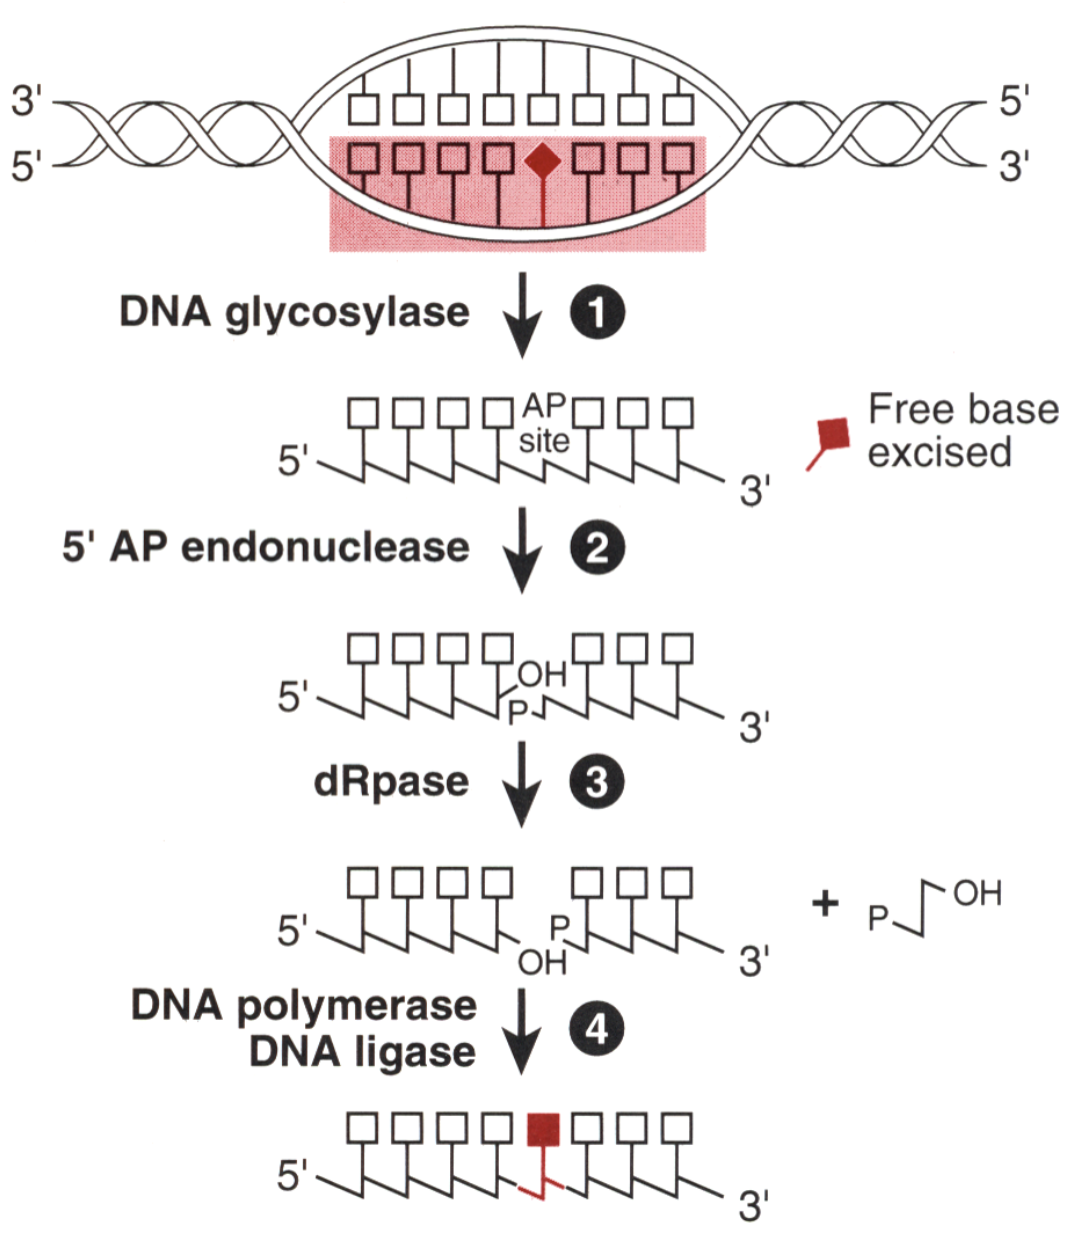
\includegraphics[width=0.98\linewidth]{../ExtFiles/DNARepaira.png}
            \caption{Base excision repair.}
            \label{fig:DNARepaira}
        \end{subfigure}
        \begin{subfigure}[b]{0.63\linewidth}
            \centering
            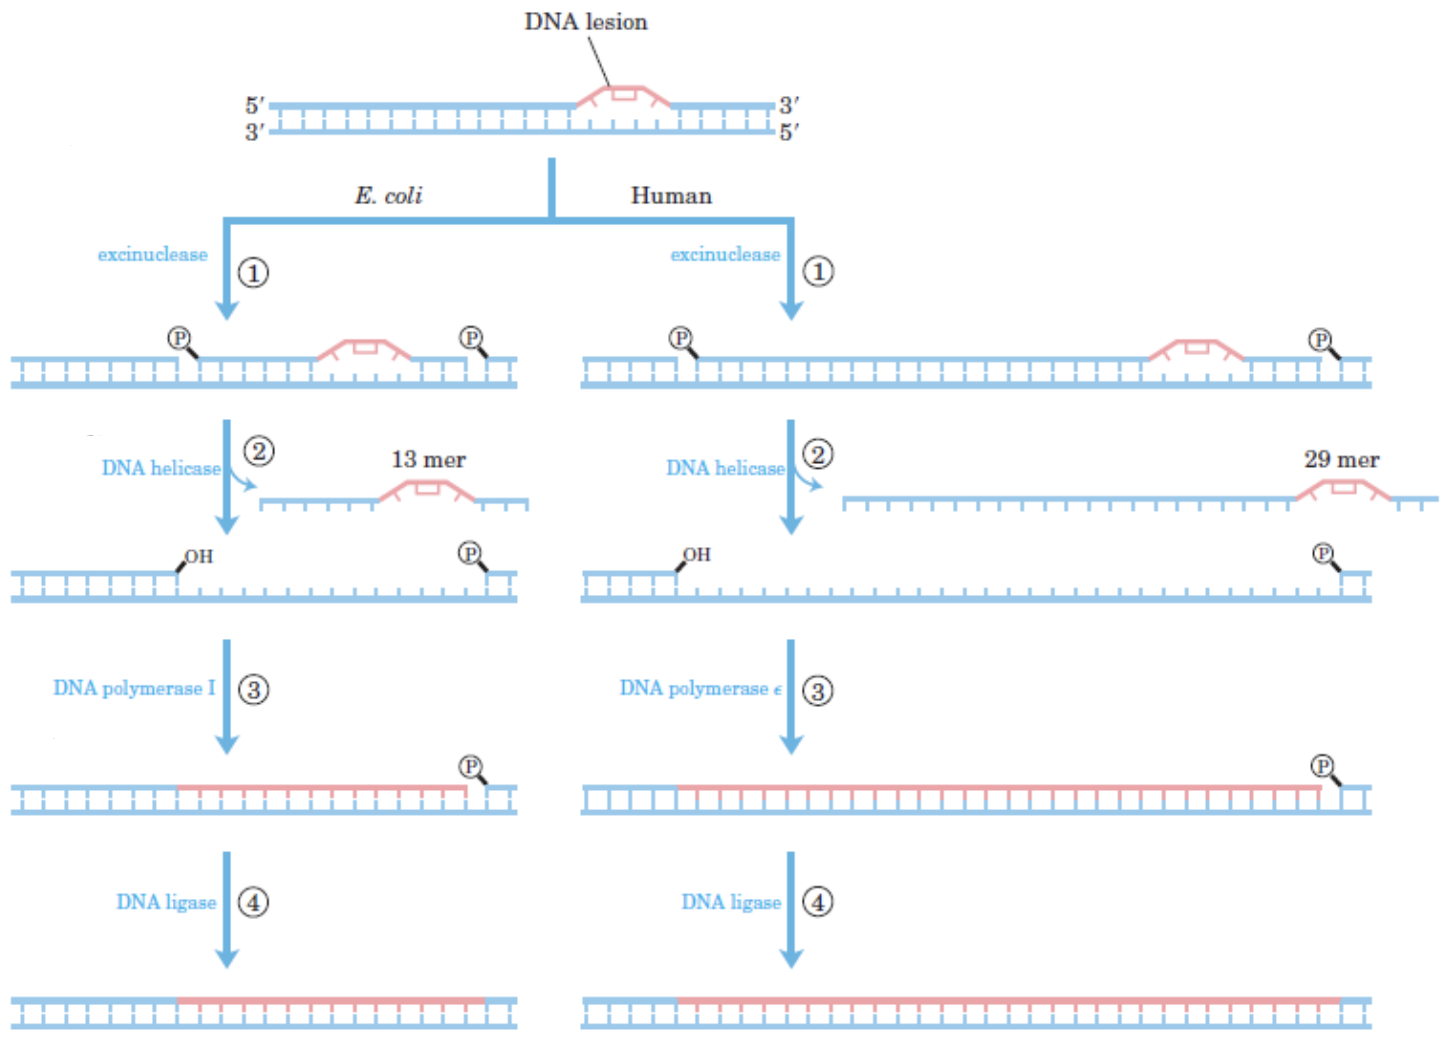
\includegraphics[width=0.9\linewidth]{../ExtFiles/DNARepairb.png}
            \caption{Nucleotide excision repair.}
            \label{fig:DNARepairb}
        \end{subfigure}
    \end{figure}
    \begin{figure}[H]
        \ContinuedFloat
        \centering
        \begin{subfigure}[b]{0.8\linewidth}
            \centering
            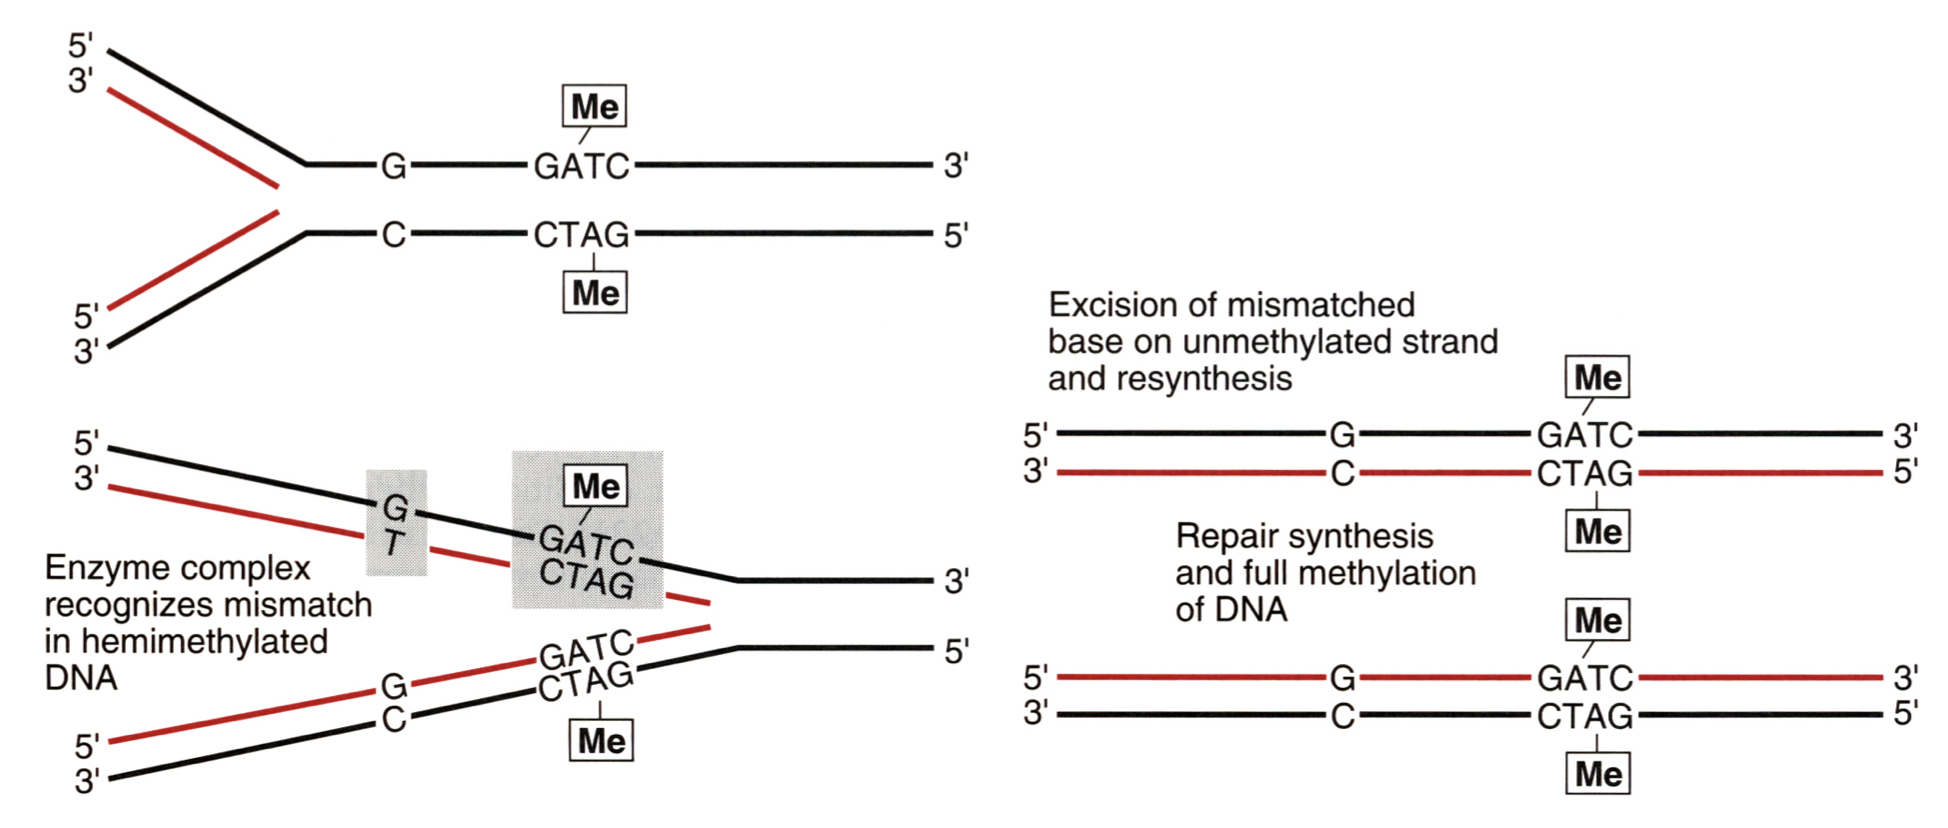
\includegraphics[width=0.9\linewidth]{../ExtFiles/DNARepairc.png}
            \caption{Mismatch repair.}
            \label{fig:DNARepairc}
        \end{subfigure}
        \caption{DNA repair strategies.}
        \label{fig:DNARepair}
    \end{figure}
    \begin{itemize}
        \item Direct reversal/repair (DR): Enzymes catalyze the reverse reaction; no removal or replacement of the base is needed. Chemically modifies what's already there (doesn't replace it with new bp's).
        \begin{itemize}
            \item The detailed mechanism of DNA phytolyases is not testable material.
        \end{itemize}
        \item Base excision repair (BER): DNA glycosylases cleave the ribose-base bond to produce apurinic/ apyrimidinic (AP) sites.
        \begin{itemize}
            \item See Figure \ref{fig:DNARepaira}.
            \item Procedure:
            \begin{enumerate}
                \item DNA glycosylases hydrolyze the N-glycosyl bond of damaged bases.
                \item This creates an "AP" site.
                \item AP endonucleases recognize the AP site and hydrolyze the phosphodiester $5'$ or $3'$ of each AP site (mostly $5'$).
                \item Exonucleases remove the backbone at free ends.
                \item DNA polymerase and ligase fill in and seal the gap.
            \end{enumerate}
            \item Most DNA glycosylases recognize a specific damaged base.
            \item In general, $<30$ kD monomeric proteins.
            \item No requirement for cofactors.
        \end{itemize}
        \item Nucleotide excision repair (NER): Enzymes remove a segment of DNA including the lesion and several nucleotides on either side.
        \begin{itemize}
            \item See Figure \ref{fig:DNARepairb}.
            \item Create nicks at two sites. Remove the DNA with lesion. Fill the gap with polymerase. Ligation via ligase.
        \end{itemize}
        \item Mismatch repair (MR): A subset of BER and NER systems that can discriminate an improper base among two normal nucleotides forming a non W-C pair.
        \begin{itemize}
            \item Most repair mechanisms are good for recognizing obvious abnormalities (e.g., uracil in DNA, paired pyrimidines, etc.). MR deals with cases when you have two pairs that don't match and it's not immediately clear which is the error.
            \item Origin of mismatched (non-W-C) natural DNA base pairs:
            \begin{itemize}
                \item DNA polymerase errors: \num{e-4} (intrinsic) $\times$ \num{e-3} (proofreading) = \num{e-7} per base per generation.
                \item Heteroduplex DNA arising from homologous recombination.
                \item Deamination of 5-Me-C to T (forming G:T pairs).
            \end{itemize}
            \item The challenge in repairing a mismatch is distinguishing the "incorrect" base among two natural bases.
            \item Methyl-directed MR.
            \begin{itemize}
                \item See Figure \ref{fig:DNARepairc}.
                \item \emph{E. coli} methylates \ce{N^6} of A in GATC ("dam" methylation).
                \item Methylation lags behind DNA replication (which always makes non-methylated DNA).
                \item 1976: B. Wagner and M. Meselson hypothesized that the lack of methylation in a newly synthesized strand allows strand discrimination during mismatch correction.
            \end{itemize}
            \item Experimental support:
            \begin{itemize}
                \item No PCR, none of today's routine bio experiments were available in the 1980s.
                \item The key experiments: Introduce into cells hemimethylated heteroduplex DNA and allow mismatch repair to take place.
                \item This occurred even if the nearest methylation site was $>1000$ bp from the mismatch!
                \item Neither strand methylated: Correction of either strand.
                \item One strand methylated: Correction of unmethylated strand.
                \item Both strands methylated: Slow correction of either strand.
            \end{itemize}
            \item Current MR model (not testable):
            \begin{itemize}
                \item MutS binds the mismatch or frameshift loop.
                \item MutS/L/H complex brings the mismatch and GATC together.
                \item MutH nicks the nonmethylated strand $5'$ of the GATC.
                \item ExoVII or RecJ degrades $5'$-$3'$ from GATC to the mismatch or Exol degrades $3'$-$5'$ from GATC to the mismatch.
            \end{itemize}
        \end{itemize}
    \end{itemize}
    \item No translation today; will be next time. The next lecture will have less content.
\end{itemize}



\section{Chemical Modifications of DNA and RNA Bases}
\begin{itemize}
    \item \marginnote{10/6:}On this year's Nobel prize in chemistry.
    \begin{itemize}
        \item Awarded for the \textbf{click reaction}.
        \item This is the \emph{key} reaction that biologists use today in their research. If you asked any chemical biologist who should have gotten this year's Nobel prize, Carolyn Bertozzi would have been on their short list.
    \end{itemize}
    \item \textbf{Click reaction}: A reaction between an azide and an alkyne that may or may not need to be accelerated by a copper iodide catalyst (depending on how strained the alkyne is).
    \begin{figure}[h!]
        \centering
        \footnotesize
        \schemestart
            \chemfig{R_1-N=\charge{90:3pt=$\oplus$}{N}=\charge{90:3pt=$\ominus$}{N}}
            \+
            \chemfig{R_2-~}
            \arrow{->[(CuI)]}
            \chemfig{[:18]*5(=(-R_2)-N=N-N(-R_1)-)}
        \schemestop
        \caption{Click reaction.}
        \label{fig:clickRxn}
    \end{figure}
    \begin{itemize}
        \item Useful in biology because it's \emph{orthogonal} to the entire biological system.
        \item Two keys:
        \begin{enumerate}
            \item It will occur in aqueous solution (unlike many organic reactions we learn about).
            \item It will not impact anything else in the biological system.
        \end{enumerate}
        \item Thus, you can use it to manipulate a specified thing in your system.
    \end{itemize}
    \item Tang cut out bioorthogonal chemistry from this year's syllabus but reconsidered the day before the Nobel was awarded; we will now have a lecture on it.
    \begin{itemize}
        \item Tang brags about predicting Nobel prizes.
        \item K. Barry Sharpless is the second chemist ever to receive two Nobel prizes. The faculty at UChicago used to debate whether or not he was worth a second Nobel; Tang bet he was, and now he is.
    \end{itemize}
    \item On the style of this class.
    \begin{itemize}
        \item Not as much of an attention to detail; instead of using 3 quarters to cover 1 book, we're building a bookcase. Every lecture is about a different topic, each of which has books written on it.
        \item In terms of testing, Tang will not test a tiny thing on her slides; it's more about the concept.
        \item She wants us to know that such research exists so that we know to read more about it if we ever need to in our research.
    \end{itemize}
    \item \textbf{DNA transcription}: A process that passes genetic information from DNA to RNA.
    \begin{itemize}
        \item RNA is synthesized by RNA polymerases using DNA as a template and NTPs as building blocks (instead of dNTPs).
        \item RNA polymerases do not require a primer (vs. DNA polymerase).
        \item RNA polymerases also elongate RNA in the $5'$-$3'$ direction.
        \item RNA polymerases lack proofreading mechanisms (vs. DNA polymerases).
        \begin{itemize}
            \item Synthesis is fairly accurate, a mistake here will likely not be repeated, and mRNA doesn't really matter.
        \end{itemize}
        \item Defining the template and nontemplate strand: The template strand does all of the heavy lifting/is directly involved in synthesis. The nontemplate/coding strand is what's replicated (i.e., what gets "all the publicity").
    \end{itemize}
    \item RNA synthesis begins at promoters.
    \begin{itemize}
        \item Similar to DNA synthesis, initiation is what's most controlled. The speed of transcription is determined by how strong the promoter, i.e., how strongly RNA polymerases are attractedl
        \item RNA polymerase binds to specific sequences in DNA (promoters), which direct the transcription of adjacent segments of DNA (genes).
        \item Consensus sequences in promoters: Affect the efficiencey of RNA polymerase binding and transcription initiation.
        \item Promoter sequence establishes a basal level of expression that can vary greatly from one \emph{E. coli} gene to the next.
        \item This bacterial example is completely different from how eukaryotes operate.
    \end{itemize}
    \item Ribosome binding site (prokaryotes)/Kozak sequence (eukaryotes) is a \textbf{promotor} at the start of RNA that binds it to the ribosomer. There's also a \textbf{terminator} site.
    \item Tang is skipping the historical exploration of translation.
    \item Translation.
    \item Nucleic acid catalysis.
    \begin{itemize}
        \item Some RNA can actually catalyze chemical reactions.
        \item Ribozymes were a hot topic in the 80s and 90s.
        \item Why study ribozimes?
        \begin{itemize}
            \item Implications for the origin of life: Prebiotic soub to RNA to proteins to simple life (links \emph{amplifiable information} to \emph{function}).
            \item RNA and proteins were a chicken-and-egg problem; this discovery suggests that RNA came first.
        \end{itemize}
        \item We haven't found natural examples of nucleic acid catalysis yet; all known examples were developed in the lab.
        \begin{itemize}
            \item Tang suggests there may be some examples in basic forms of life.
        \end{itemize}
        \item How do nucleic acids catalyze reactions compared with proteins?
        \begin{itemize}
            \item All known all-RNA catalysts in nature accelerate phosphoryl transfer reactions (forming or breaking phosphodiester bonds).
        \end{itemize}
        \item More info in slides.
    \end{itemize}
    \item \textbf{Ribozyme}: Catalytic RNA; short for ribonucleic acid enzyme.
    \item \textbf{Aptamer}: A receptor; the analogous function in proteins is antibodies (binding but not causing a reaction).
    \item \emph{Tetrahymena} Catalytic RNA.
    \begin{figure}[h!]
        \centering
        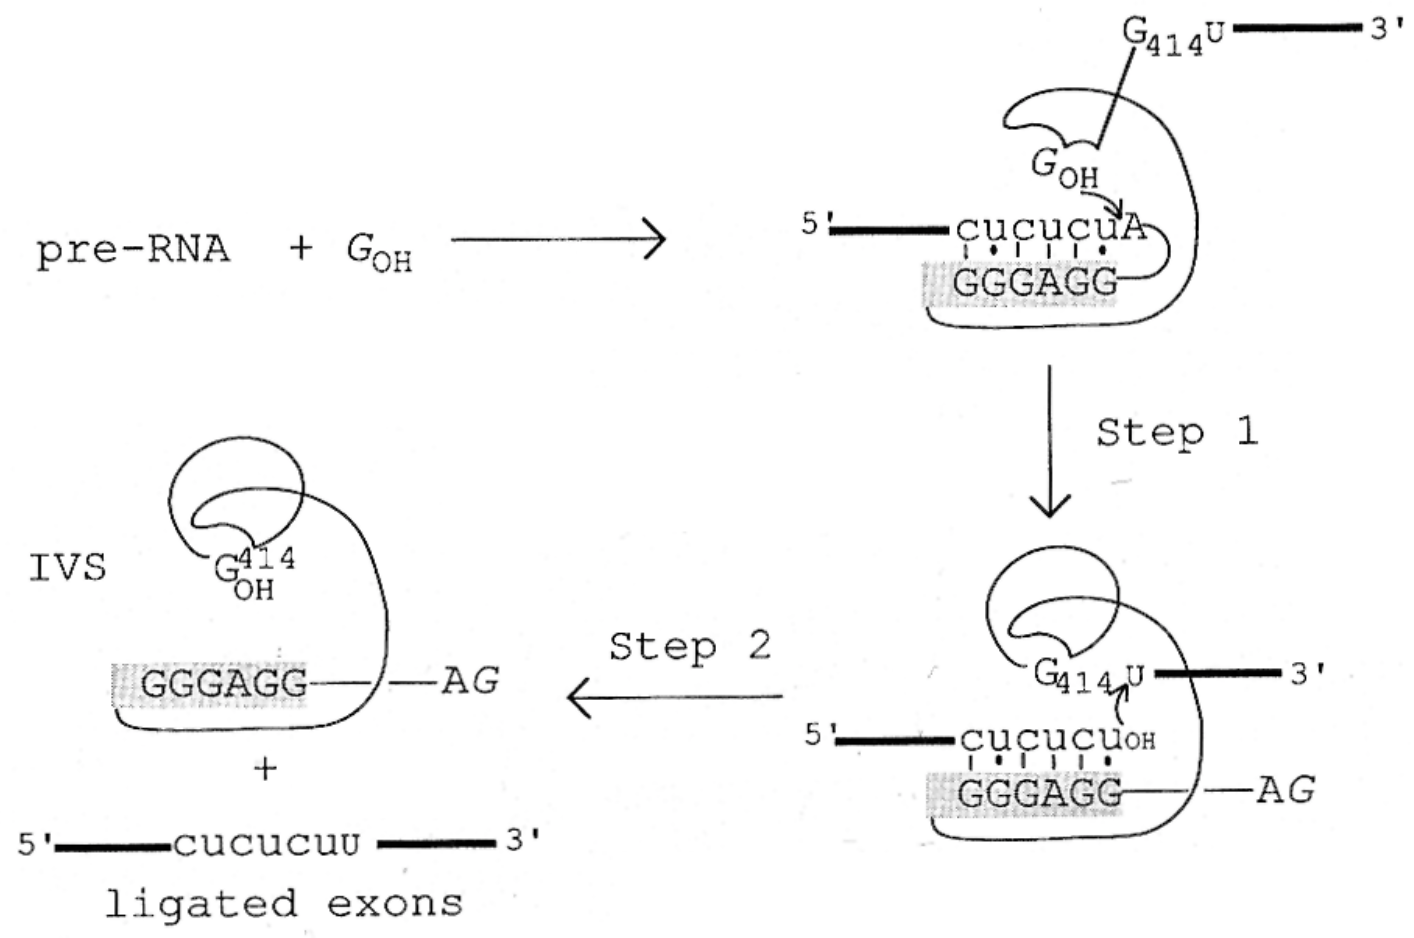
\includegraphics[width=0.6\linewidth]{../ExtFiles/catalyticRNA.png}
        \caption{Catalytic RNA.}
        \label{fig:catalyticRNA}
    \end{figure}
    \begin{itemize}
        \item Discovered 1981; Nobel Prize 1989.
        \item \emph{Tetrahymena thermophilia} is a highly heat resistant form of life. Their pre-ribosomal RNA (pre-rRNA) can catalyze its own splicing, yielding an interveining sequence (IVS) and a mature rRNA via two phospho-transesterifications.
        \item More details on the mechanism:
        \begin{itemize}
            \item Catalyzed by GTP (or GMP, but slower this way).
            \item The RNA folds, engages GTP. This enables GTP to insert itself, cleaving the RNA. Now there is a sequence that is only attached to the rest of the RNA by hydrogen bonding.
            \item The partially free RNA pice adds more of the original RNA to itself and finally detaches.
        \end{itemize}
        \item Tom Cech (discoverer) believed that protein was catalyzing the reaction.
        \begin{itemize}
            \item Tried denaturing enzymes and heat, but the reaction still proceeded. Strongly suggested it wasn't a protein, but couldn't confirm it wasn't a heat-resistant or otherwise very stable protein (or trace amounts of a highly efficient protein catalyst).
            \item Final clue: Went to an \emph{in vitro} system. Did \emph{in vitro} transcription to get the RNA and RNA only (the material is no longer distilled from the organism), dumped that into the reaction, added the substrate, and watched it occur.
            \item Took them a year.
        \end{itemize}
    \end{itemize}
    \item \emph{Tetrahymena} Ribozyme Structure.
    \begin{itemize}
        \item The X-ray crystal structure was solved to a decent resolution (\SI{2.8}{\angstrom} --- atomic resolution) for one domain of the catalytic core, and to \SI{5}{\angstrom} for the entire core.
        \begin{itemize}
            \item Nowadays, you will not be able to publish resolution as low as \SI{5}{\angstrom}.
            \item This was Jennifer Doudna's first paper as an independent researcher!
        \end{itemize}
        \item Combination of structural and biochemical studies suggests a mechanism mediated by several bound magnesium cations.
        \begin{itemize}
            \item Emphasizes that nucleic acid reactions often need to be catalyzed by ions.
        \end{itemize}
        \item Take home lesson: RNA can fold into compact, protein-like structures.
    \end{itemize}
    \item Structure of (most of) the ribosome.
    \begin{itemize}
        \item Nobel prize (2009) --- many scientists tried and failed for years, but they finally got it in 2009.
        \item The ribosome is the cell's way of converting genetic information into molecular structure and chemical function.
        \item Bacterial ribosome: Huge --- 2.6 million Da (far bigger than glycosylase), 2/3 RNA (3 total), 1/3 protein (55 total), two subunits (50S and 30S).
        \begin{itemize}
            \item You can delete some of the proteins and it will still function, but you cannot delete any of the RNA.
        \end{itemize}
    \end{itemize}
    \item Video that Tang saw as a grad student that really impressed her and she wants to share with us (\href{https://youtu.be/RedO6rLNQ2o}{link}).
    \item The ribosome is a ribozyme.
    \begin{itemize}
        \item The reaction that the ribosome catalyzes is carried out almost entirely by RNA (that's what the ribosome active site is made of).
        \item Details of the protein building reaction.
        \begin{itemize}
            \item There are three sites in the ribosome: The exit, peptodyl, and aminoacyl site. The tRNA comes in at the A site and exits at the P site. At the E site, the tRNA has already been utilized.
            \item The incoming amine group does a nucelophilic attack on the tRNA-bound ester group of the amino acid added just before.
            \item This kicks out the ester-bound tRNA, and everything shifts down a site.
            \item A new codon is exposed at the aminoacyl site, and a new tRNA plust amino acid binds to it.
            \item This process repeats over and over again, 3 RNA at a time, building a longer and longer peptide chain.
        \end{itemize}
        \item A transition state mimic that scientists use to get the crystal structure of the active state of the ribosome is CCdAp-Puromycin.
        \begin{itemize}
            \item Puromycin is a useful antibiotic used to inhibit protein synthesis.
            \item Puromycin doesn't break, so we can make the ribosome get stuck in the transition state.
        \end{itemize}
        \item Tang goes over the electron pushing of the protein building reaction, as seen in Figure \ref{fig:ribosomeBuildProtein}.
    \end{itemize}
    \item Mechanism of the ribosome.
    \begin{figure}[h!]
        \centering
        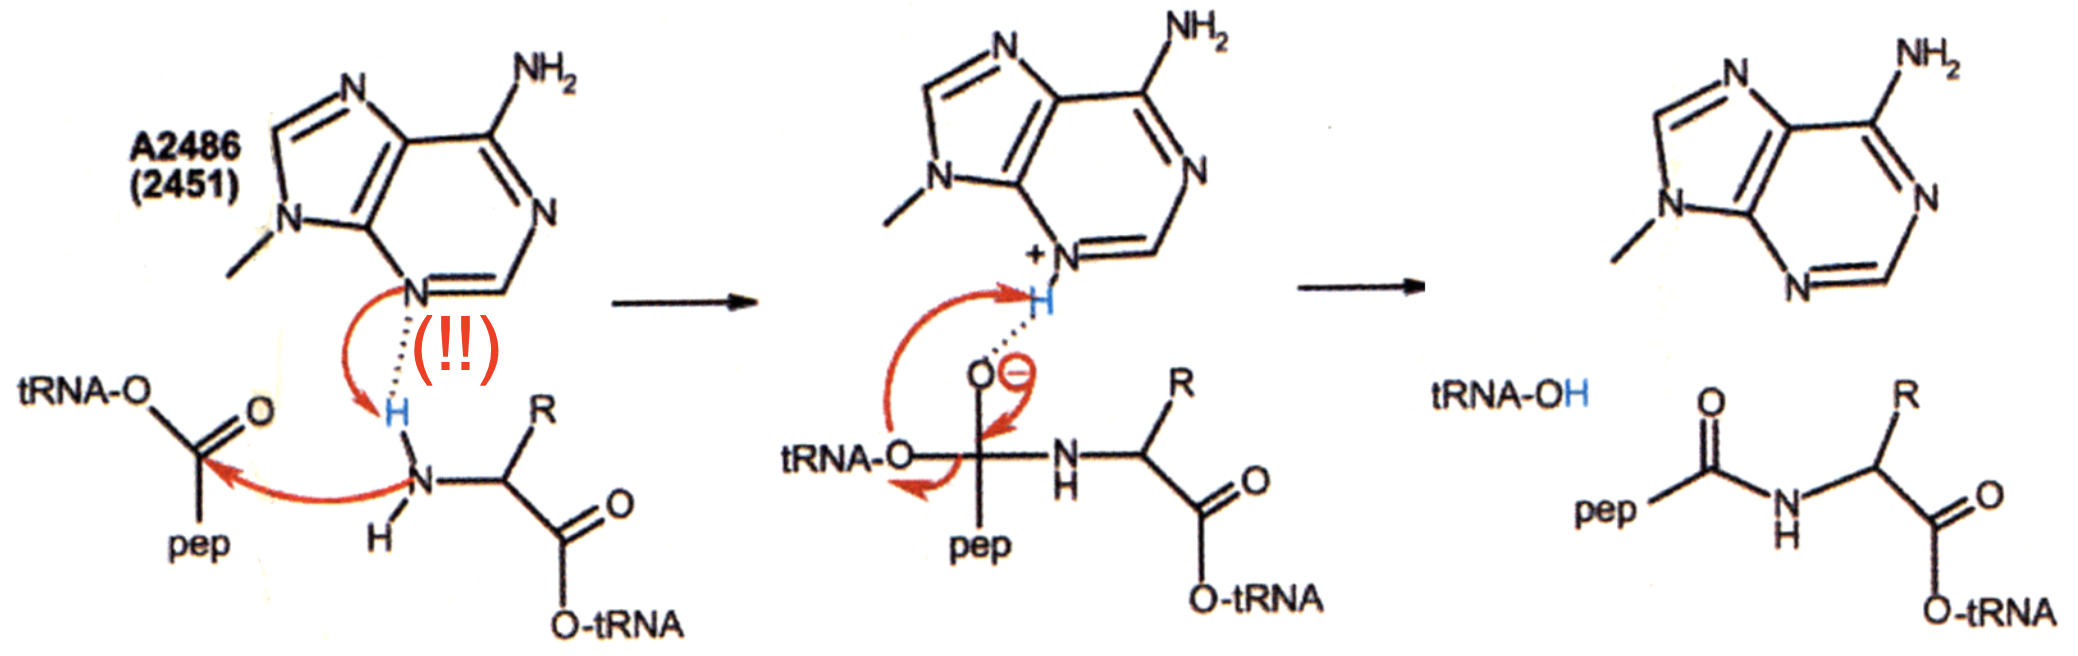
\includegraphics[width=0.7\linewidth]{../ExtFiles/ribosomeMechanism.png}
        \caption{Mechanism of the ribosome.}
        \label{fig:ribosomeMechanism}
    \end{figure}
    \begin{itemize}
        \item Recall from lecture 2 that at physiological $\pH$, no nucleobases are charged. You have to go to $\pH\approx 3$ for protonation or $\pH\approx 10$ for deprotonation. This implies that nucleobases are really terrible acid-base catalysts.
        \item Yet we do have a proton transfer occuring from the incoming amino acid to the exiting tRNA.
        \item The XPS crystal structure implies that A2486 catalyzes the proton-transfer reaction.
        \item N1 is the site on adenine that can most easily be protonated, but N3 is closest to the carbonyl O and the incoming amine, so it is active as the catalyst.
        \item But N3 has $\pKa\approx 1.5$, implying that if you have an isolated adenine, you need to drop the $\pH$ to 1 before you can get protonation.
        \item How does this work? We have a complex hydrogen-bonding network that delocalizes a negative phosphate charge to a neighboring guanine that, in turn, passes it to A2486 to aid in its deprotonation effort. The effect is that actual $\pKa$ of AdeN3 is 7.6, up six orders of magnitude due to the H-bonding interactions.
        \item If tested on this, we'll be given information on the hydrogen bonding network. We likely won't be tested on it, though.
    \end{itemize}
    \item Slides on RNA ligase will not be tested: It's one of Tang's favorite topics, but it falls under directed evolution.
    \item Now for lecture 4 content.
    \item Will modification always change DNA or RNA always affect W-C interactions?
    \begin{itemize}
        \item The most frequent modification (5-methylation) does not change base pairing, but it does affect interaction with proteins.
        \item Today: Modifications that show up naturally but don't necessarily cause modifications.
        \item This lecture will be shorter: Tang shoots to finish today.
    \end{itemize}
    \item Overview.
    \begin{itemize}
        \item Diverse natural base modifications in DNA and RNA and their biological functions.
        \item Epigenetics: All cells have the same set of DNA, but different cells can behave very differently. This is caused by epigenetics.
        \item Epitranscriptomics describes modifications on mRNA. One example: $N^6$-methyladenosine (m\textsuperscript{6}A).
        \item If time allows: The arms race of base modifications in bacteria and phages.
    \end{itemize}
    \item Natural DNA base modifications.
    \begin{itemize}
        \item Most installed by enzymes (sometimes, phages directly use modified dNTP to synthesize their genome, but that's beyond the scope of this class; for now, most means always).
        \item Not always required for survival, but can lead to an evolutionary advantage (recall from last time the example of mismatch correction based on methylation; bacteria that can't do this have a much higher mutation rate).
        \item Modifications occur at specific locations on the four cananonical bases.
        \begin{itemize}
            \item Adenine: C2 and $N^6$.
            \item Cytosine: C5 and $N^4$.
            \item Guanine: N7.
            \item Thymine: $C^5$.
            \item Exceptions exist, but we won't discuss them.
        \end{itemize}
        \item 1.5\% of our genome (5\% of cytosine) is 5-methylcytosine.
        \item 5-(hydroxymethyl)cytosine, 5-formylcytosine, and 5-carboxycytosine are also possible in humans, in decreasing frequency.
        \item Other stranger modifications (such as bonding sugars to C5) can occur in lower organisms.
        \item Uracil can also be hydroxymethylated and formylated. Base J is uracil with a sugar at C5.
        \item $N^6$-methyladenine is very abundant in bacteria, but there is a huge contraversy over whether or not it is in humans.
        \item We don't need to memorize any of these save 5-methylcytosine.
    \end{itemize}
    \item Detecting DNA modifications: Use LC-MS/MS.
    \begin{itemize}
        \item Harvest the DNA, digest it into individual nucleotides, get rid of the phosphate, shoot it into a mass spectrometer, and see if you can detect the modified base.
        \item Restriction: Rare modifications can fall below the detection limit.
        \item Point of contraversy: The second and third steps above are accomplished using enzymes from prokaryotes, but these can leech bacterial DNA nucleotides.
        \begin{itemize}
            \item Errors regarding this can account for some of the false positive detections of $N^6$-methyladenine in eukaryotic DNA.
        \end{itemize}
        \item We will see beter methods of sequencing later.
    \end{itemize}
    \item Epigenetics and DNA methylation.
    \begin{itemize}
        \item Epigenetics is the study of heritable phenotype changes that do not involve alterations in the DNA sequence. Two big areas: Modification of DNA and modification of histone proteins.
        \item 5mC is the "5th richest" base in human DNA. Happens primarily within CpG islands in promoters. Most often correlated with gene suppression.
    \end{itemize}
    \item DNA methylation is dynamic.
    \begin{figure}[h!]
        \centering
        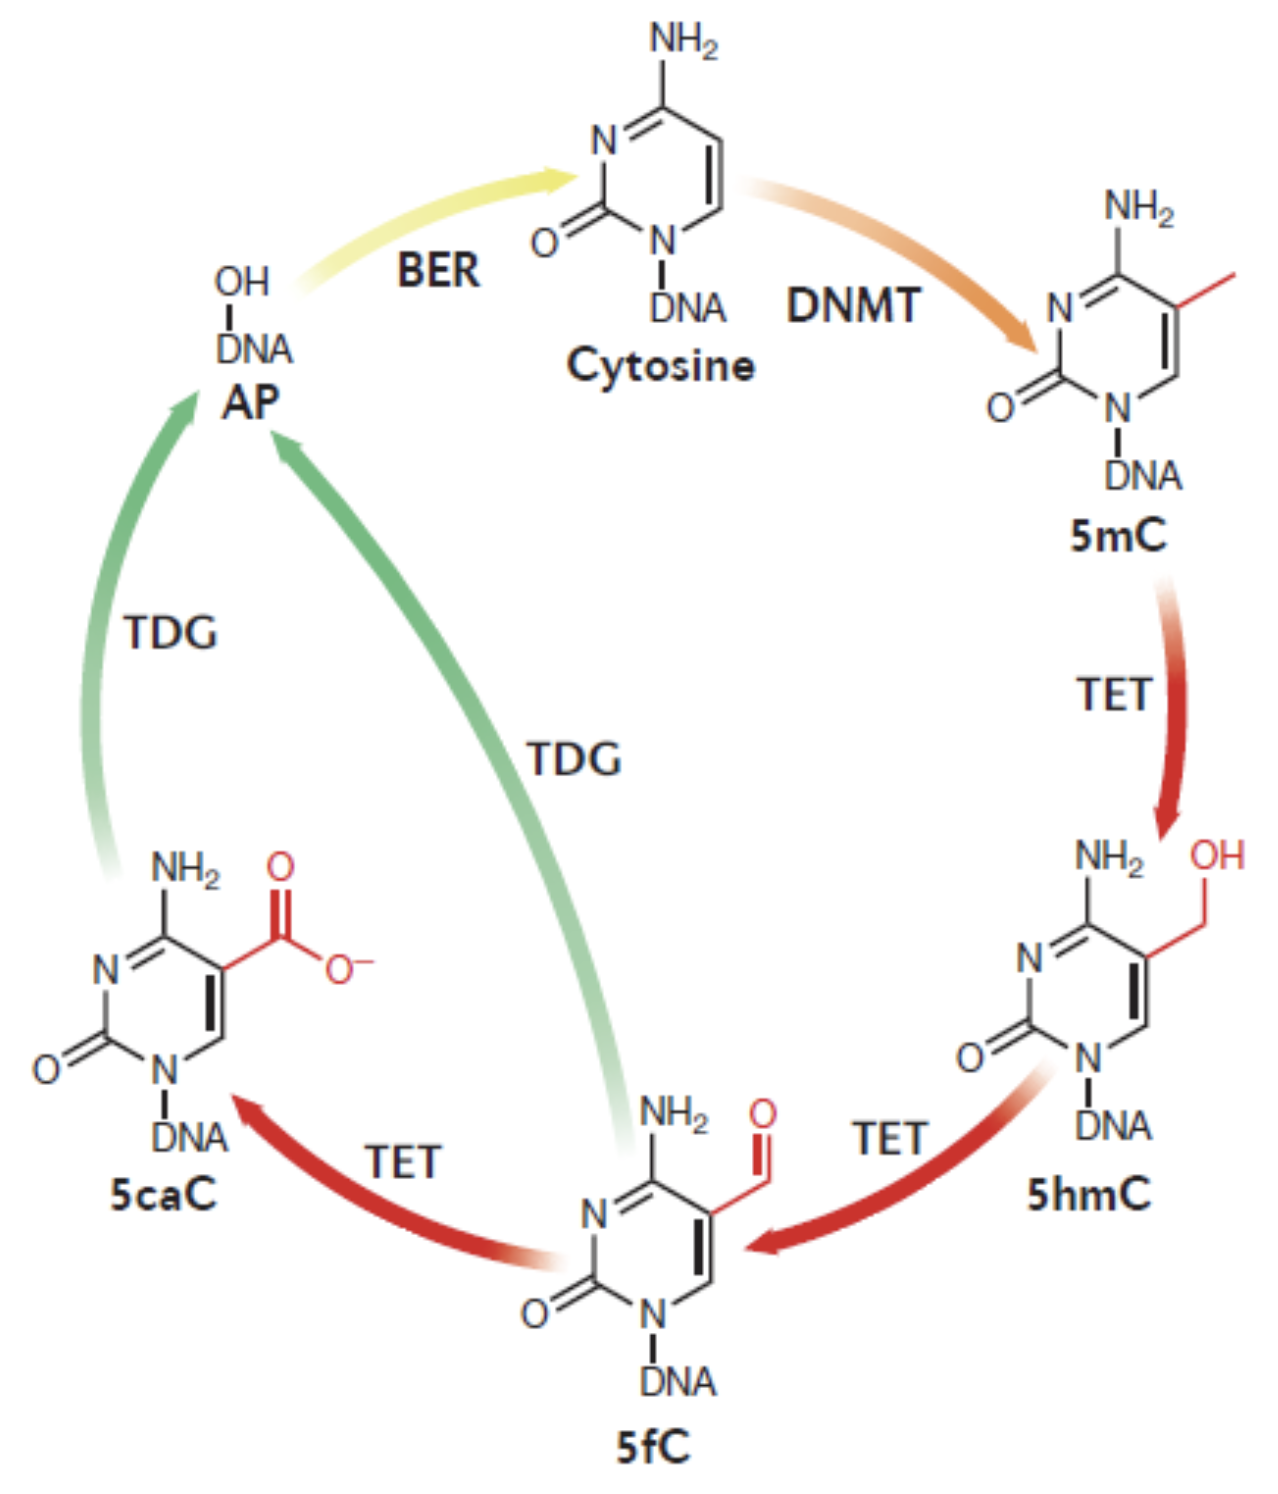
\includegraphics[width=0.4\linewidth]{../ExtFiles/activeMeth.png}
        \caption{Active methylation cycle of cytosine.}
        \label{fig:activeMeth}
    \end{figure}
    \begin{itemize}
        \item Two ways to get rid of modified bases:
        \begin{itemize}
            \item The passive way, i.e. if we never replace the methylation marks after DNA replication (recall from the discussion associated with Figure \ref{fig:DNARepairc} that newly synthesized DNA is unaltered). If modifications are never regenerated, they will slowly become less and less common, only occuring in the original strand that has now been duplicated and "diluted" many times.
            \item Active demethylation: Catalyzed by the TET family in eukaryotes.
        \end{itemize}
        \item 5mC and 5hmC have different effects on gene transcription (5hmC is more activating than repressing).
        \item 5mC and 5hmC are viewed as modifications; 5fC and 5caC are viewed as lesions and will be fixed. We will not be tested on this, though.
        \item Histone marks can have very different functions (acetylation vs. methylation).
        \item Epigenetics is a huge research field and waiting for a Nobel prize.
    \end{itemize}
    \item 5mC/5hmC in early embryonic development.
    \begin{itemize}
        \item Two scenarios: Skin/liver cells are still dividing but are at their terminal epigenetic state; a fertilized egg is still diversifying. The fertilized egg has more motivation to change its epigenetics.
        \item Thus, throughout development, you see a quick decrease in 5mC and some waves in 5hmC.
    \end{itemize}
    \item DNA methylation on aging and cancers.
    \begin{itemize}
        \item Not tested, but interesting.
        \item DNA methylation maps change with chronological age. When you are born, you have the most beautiful epigenetics; it gets messed up as you age.
    \end{itemize}
    \item How to detect 5mC/5hmC sites in DNA?
    \begin{figure}[h!]
        \centering
        \footnotesize
        \begin{tikzpicture}[
            every node/.style={inner sep=5pt}
        ]
            \node (2)              {- C - C - C - C - {\color{rex}C} - C - C - C - C - C -};
            \node (1) [below=of 2] {- C - C - C - C - {\color{rex}\ce{{}^mC}} - C - C - C - C - C -}
                edge [->] node[right]{sequencing} (2)
            ;
            \node (3) [below=of 1] {- U - U - U - U - {\color{rex}\ce{{}^mC}} - U - U - U - U - U -}
                edge [<-] node[right]{bisulfite} (1)
            ;
            \node (4) [below=of 3] {- U - U - U - U - {\color{rex}C} - U - U - U - U - U -}
                edge [<-] node[right]{sequencing} (3)
            ;
        \end{tikzpicture}
        \caption{Bisulfite chemistry.}
        \label{fig:bisulfite}
    \end{figure}
    \begin{itemize}
        \item Bisulfite chemistry.
        \begin{itemize}
            \item One of Tang's favorite topics in biochemistry; will definitely be tested.
        \end{itemize}
        \item When you mix DNA with bisulfite and heat it up, cytosine converts to uracil. Since uracil pairs with thymine, you will detect thymine when you should detect guanine if you do the bisulfite treatment.
        \item If you have 5mC, bisulfite won't attack for steric reasons, so 5mC remains unchanged.
        \item Thus, between the original strand and the bisufited strand, you get differentiation.
        \item Whichever cytosines don't change before and after bisulfiting are your methylated C's.
        \begin{itemize}
            \item Notice how in Figure \ref{fig:bisulfite}, the only cytosine which doesn't change in between the two rounds of sequencing is the methylated one, indicated in bright red.
        \end{itemize}
        \item Assuming the reaction yield of bisulfite chemistry is 100\%. What if the yield is 50\%? We are lucky here: Bisulfite chemistry is 99.9\% efficient, so the number of false positives is very low.
    \end{itemize}
    \item If you want to detect beyond 5mC, there are more complex methods; she won't test us on these though.
    \item Natural RNA base modifications.
    \begin{figure}[h!]
        \centering
        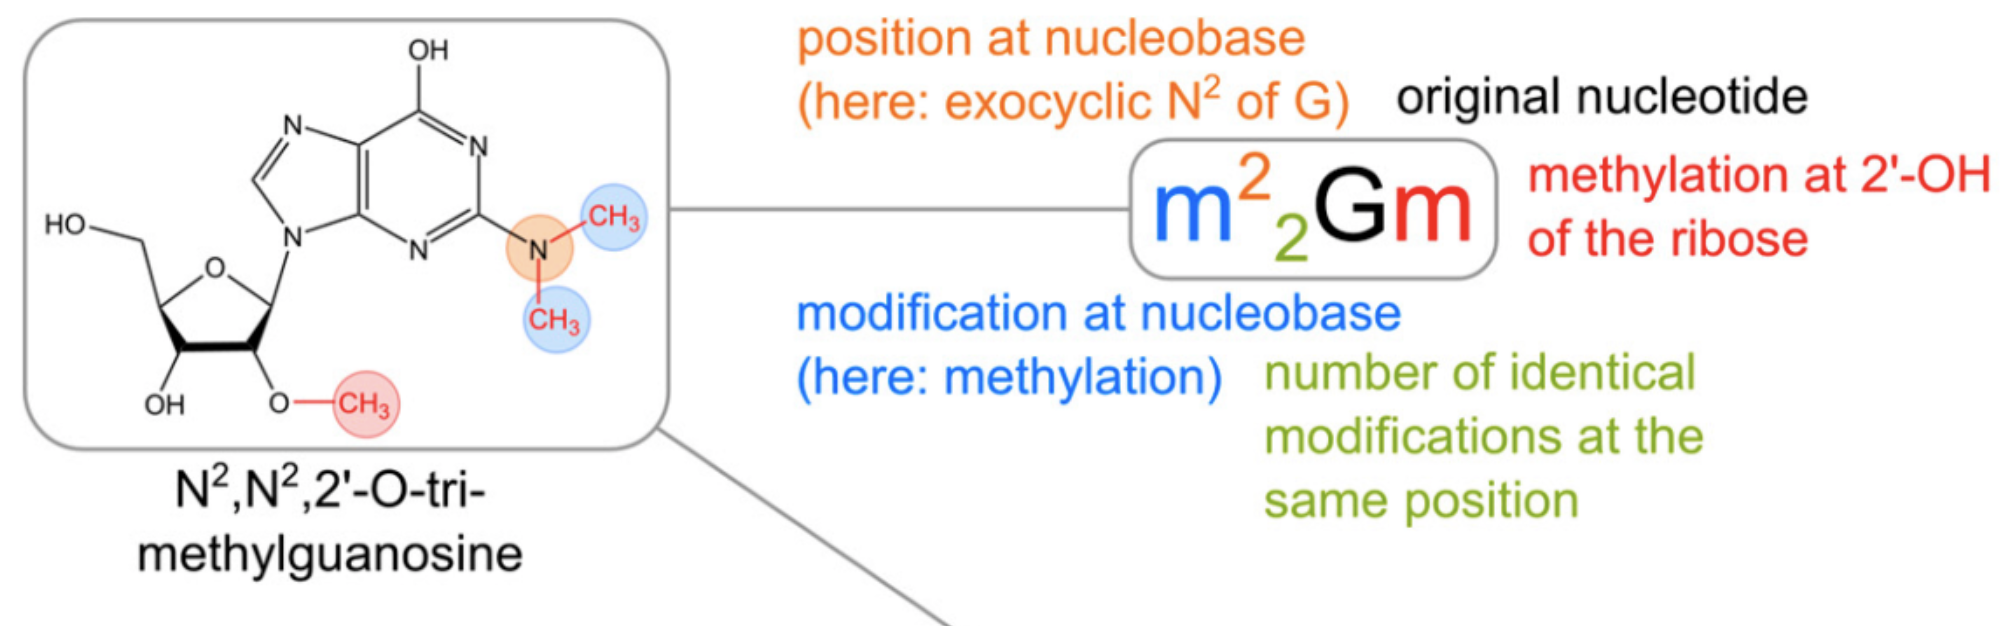
\includegraphics[width=0.7\linewidth]{../ExtFiles/RNAbaseModName.png}
        \caption{Naming convention for RNA base modifications.}
        \label{fig:RNAbaseModName}
    \end{figure}
    \begin{itemize}
        \item If you compare between DNA and RNA base modifications, you will find DNA boring.
        \item There are 20 known DNA base modifications; there are over 150 known RNA ones, and many look very weird.
        \item Naming convention for base modifications: See Figure \ref{fig:RNAbaseModName}.
        \item RNA base modificatinos occur in all three major RNA species (tRNA, mRNA, and rRNA) and in other RNA species such as snRNA and miRNA.
        \item They are found in all three domains (archaea, bacteria, and eukarya). Some modifications are unique to a single domain.
    \end{itemize}
    \item tRNA is heavily modified.
    \begin{itemize}
        \item $>75\%$ of RNA modifications are present in tRNA.
        \item tRNA are typically less than 100 nucleotides long, so the density of modifications is very high.
        \item These modifications enhance translation.
    \end{itemize}
    \item \textbf{Transcriptome}: The set of all RNA within a cell.
    \item \textbf{Epitranscriptome}: The set of all biochemical modifications to all RNA.
    \item Epitranscriptome and mRNA methylation.
    \begin{itemize}
        \item Epitranscriptomics defines the half-life of RNA and determines how strongly mRNA gets translated.
        \item In many papers about base modifications, it's evident that the figures are not drawn by chemists (there are obvious mistakes such as missing charges, wrong atoms, etc.).
    \end{itemize}
\end{itemize}




\end{document}